%%=============================================================================
%% Methodologie
%%=============================================================================

\chapter{Methodologie}
\label{ch:methodologie}
\lstset{
    tabsize = 4, %% Sets tab space width.
    showstringspaces = false, %% Prevents space marking in strings, string is defined as the text that is generally printed directly to the console.
    numbers = left, %% Displays line numbers on the left.
    commentstyle = \color{green}, %% Sets comment color.
    keywordstyle = \color{blue}, %% Sets  keyword color.
    stringstyle = \color{red}, %% Sets  string color.
    rulecolor = \color{black}, %% Sets frame color to avoid being affected by text color.
    basicstyle = \small \ttfamily , %% Sets listing font and size.
    breaklines = true, %% Enables line breaking.
    numberstyle = \tiny,
}

%%\begin{lstlisting}[language = Java , frame = trBL , firstnumber = last , escapeinside={(*@}{@*)}]
%%public class Factorial
%%{
%%public static void main(String[] args)
%%{   final int NUM_FACTS = 100;
%%for(int i = 0; i < NUM_FACTS; i++)
%%System.out.println( i + "! is " + factorial(i));
%%}
%%
%%public static int factorial(int n)
%%{   int result = 1;
%%for(int i = 2; i <= n; i++) (*@\label{for}@*)
%%result *= i;
%%return result;
%%}
%%}
%%\end{lstlisting}


%% TODO: Hoe ben je te werk gegaan? Verdeel je onderzoek in grote fasen, en
%% licht in elke fase toe welke stappen je gevolgd hebt. Verantwoord waarom je
%% op deze manier te werk gegaan bent. Je moet kunnen aantonen dat je de best
%% mogelijke manier toegepast hebt om een antwoord te vinden op de
%% onderzoeksvraag.

% TODO: uitleg wat we allemaal nodig hebben, producer uitleggen, consumer uitleggen, 3 verschillende groottes uitleggen.
Om te testen welke van de technologieën die in dit onderzoek aan bod komen nu eigenlijk het beste is, zou je met veel zaken rekening moeten houden. Wat het beste is hangt vooral af van welke soort data je gebruikt. Ook de hoeveelheid transformaties die je data ondergaan voor dat ze uitgelezen worden of verzonden speelt een grote rol. Natuurlijk is het moeilijk om binnen de tijdspanne die er is voor dit onderzoek al deze factoren te gaan onderzoeken. Daarom zal dit onderzoek zich toespitsen op een bepaald scenario en daar conclusies uit trekken. Voor het scenario beslissen we op voorhand voor welk formaat van de data dat we dit onderzoek zullen voeren, dit zal een Json zijn. Ook zullen we het onderzoek drie keer uitvoeren, voor verschillende groottes van data. Een keer met 10 000, 100 000 en 1 000 000.  
\section{Producer project}
Het opzetten van een omgeving is per technologie verschillend. Elk heeft zijn eigen manier om data te verzenden en te ontvangen. Hieronder wordt eerst eens per technologie de implementatie getoond hoe we het project opgezet hebben. Daarna wordt er uitgelegd hoe we gaan testen welke nu de beste zal zijn. De reden waarom we specifiek deze technologieën gekozen hebben om te vergelijken kan opnieuw gelezen worden in de Stand van Zaken en de Inleiding.  

Natuurlijk moet er iets gelijkaardigs zijn om te kunnen vergelijken. Het data object dat we zullen verzenden en ontvangen bij zowel \emph{Kafka}, \emph{RabbitMq} en \emph{Google Pub/Sub} zal hetzelfde zijn. Op deze manier is het toekomstige resultaat niet afhankelijk van het type data. Dit onderzoek zal zich dus toespitsen op data met het type Json. Deze klasse (Data.class) hergebruiken we in elke technologie. Deze klasse stelt het type voor van het bericht dat we verzenden.
\begin{lstlisting}[language = Java , frame = trBL , firstnumber = last , escapeinside={(*@}{@*)}]
@Getter
@AllArgsConstructor
@NoArgsConstructor
@ToString
public class Data {
    private int id;
    private String name;
    private String description;
    private Date sendedDate;
}
     \end{lstlisting}
     
Deze klasse bevat vier attributen. Dit is om een Json object na te bootsen. Het is vanzelfsprekend dat deze klasse niet zo maar automatisch kan omgezet worden naar een Json. De manier waarop dit gedaan wordt is opnieuw per technologie verschillend. De uitleg zal gegeven worden in de subsectie van de technologie zelf. De attributen die hier gebruikt worden zijn: een id van het type int, dit is om elk data object van elkaar te kunnen onderscheiden tijdens het verzenden. Als tweede zie je name van het type String. Dit heeft als bedoeling opnieuw om verschillende objecten van elkaar te kunnen onderscheiden en om een realistisch attribuut te geven aan het Data-object. Deze doelstelling is dezelfde voor het attribuut description van het type String. Als laatste hebben we de sendedDate van het type Date. Deze zal de datum en het tijdstip bijhouden wanneer het object verzonden is. Dit zal later nog eens aangehaald worden wanneer we deze objecten genereren. 

Als u boven de klasse kijkt dan ziet u nog vier annotaties staan. Deze kunnen we gebruiken door de library van Lombok. Dit werd mogelijk gemaakt door deze dependency toe te voegen aan onze pom.xml want het gebruikte project voor dit onderzoek maakt gebruik van Maven om libraries toe te voegen.

\begin{lstlisting}[language = xml , frame = trBL , firstnumber = 1 , escapeinside={(*@}{@*)}]
<dependency>
<groupId>org.projectlombok</groupId>
<artifactId>lombok</artifactId>
<optional>true</optional>
</dependency>
\end{lstlisting}

De library Lombok geeft op voorhand al enkele handige implementaties. De gebruikte annotaties zullen we uitleggen, want natuurlijk bestaan er meer dan enkel deze die dit onderzoek gebruikt. Voor de andere mogelijkheden verwijs ik u graag door naar de site van Project Lombok waar u alle mogelijkheden op een rijtje ziet: https://projectlombok.org/features/all. 

De eerste annotatie is @Getter, deze zorgt ervoor zoals de naam al doet vermoeden, dat er voor ieder attribuut een getter aanwezig is. Op deze manier staat uw code niet overvol met getters van al uw attributen. In deze klasse zijn er niet zo veel attributen dus zou het aantal getter nog meevallen. Maar u kan zich wel inbeelden dat in een groter project in een klasse met veel attributen en andere methodes dat dit een handige annotatie is. Je ziet dus niet dat de getters aanwezig zijn maar die zijn er wel effectief. Laten we de tweede en de derde samen bekijken: @AllArgsConstructor en @NoArgsConstructor. Deze zorgen ervoor dat er een constructor gegenereerd wordt met respectievelijk al de attributen en zonder de attributen. Dit zijn vaak voorkomende constructors en het is handig om ook hiervoor een annotatie te hebben. De laatste  is de @ToString. Deze werd gebruikt tijdens het testen van het project. Dit zorgt voor een String-representatie van het object. Dit was handig om lokaal te testen. Het data object werd dan uitgeprint tijdens het verzenden om te controleren of het object wel de juiste waardes bevatte.
\subsection{Kafka}
In figuur 3.1 ziet u welke configuratie de topic heeft. Er wordt gebruik gemaakt van zes partities en de data wordt vier weken bijgehouden. Met andere woorden: als de data op de topic komt, en deze niet binnen de vier weken door een consumer gelezen wordt, dan wordt de data verwijderd en kan deze data niet meer opnieuw uitgelezen worden.
\begin{figure}[h!]
    \centering
    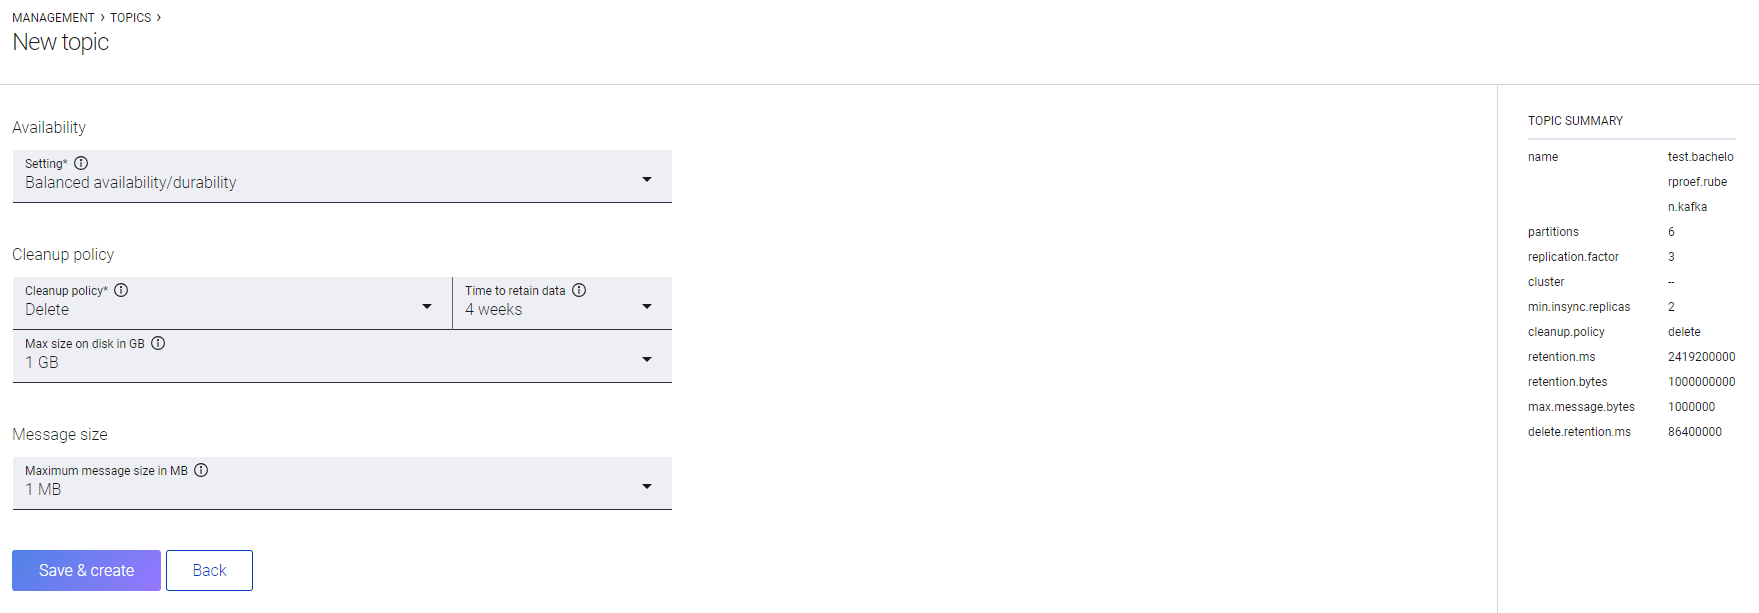
\includegraphics[width=140mm]{../kafkaConfig.png}
    \caption{Configuratie van de topic}
    
\end{figure}
\subsubsection{KafkaConfig}
Zo ziet de implementatie van de KafkaConfig.class eruit.

    \begin{lstlisting}[language = Java , frame = trBL , firstnumber = 1 , escapeinside={(*@}{@*)}]
    @Configuration
    public class KafkaConfig {
        
        @Bean
        @Primary
        public KafkaProperties kafkaProperties(
        @Value("${kafka_key}") final String kafkaKey,
        @Value("${kafka_secret}") final String kafkaSecret,
        @Value("${kafka_bootstrap}") final String kafkaBootstrap
        
        ) {
            KafkaProperties kafkaProperties = new KafkaProperties();
            
            KafkaProperties.Producer producer = kafkaProperties.getProducer();
            
            producer.getProperties().put(ProducerConfig.KEY_SERIALIZER_CLASS_CONFIG, "org.apache.kafka.common.serialization.StringSerializer");
            producer.getProperties().put(ProducerConfig.VALUE_SERIALIZER_CLASS_CONFIG, "org.springframework.kafka.support.serializer.JsonSerializer");
            
            producer.getProperties().put(ProducerConfig.BOOTSTRAP_SERVERS_CONFIG, kafkaBootstrap);
            producer.getProperties().put(ProducerConfig.RETRIES_CONFIG, "0");
            producer.getProperties().put(ProducerConfig.ACKS_CONFIG, "all");
            producer.getProperties().put(ProducerConfig.RETRY_BACKOFF_MS_CONFIG, "1000");
            producer.getProperties().put(ProducerConfig.REQUEST_TIMEOUT_MS_CONFIG, "30000");
            producer.getProperties().put(ProducerConfig.LINGER_MS_CONFIG, "200");
            kafkaProperties.getProperties().put(SslConfigs.SSL_ENDPOINT_IDENTIFICATION_ALGORITHM_CONFIG, "https");
            kafkaProperties.getProperties().put(SaslConfigs.SASL_MECHANISM, "PLAIN");
            kafkaProperties.getProperties().put("request.timeout.ms", "20000");
            kafkaProperties.getProperties().put("retry.backoff.ms", "500");
            kafkaProperties.getProperties().put(SaslConfigs.SASL_JAAS_CONFIG, "org.apache.kafka.common.security.plain.PlainLoginModule required username=\""
            + kafkaKey + "\" password=\"" + kafkaSecret + "\";");
            kafkaProperties.getProperties().put("security.protocol", "SASL_SSL");
            
            kafkaProperties.getProperties().put(JsonSerializer.ADD_TYPE_INFO_HEADERS, "false");
            
            return kafkaProperties;
        }
            \end{lstlisting}
            
     In deze klasse ziet u dat het instellen van de nodige properties in de kafkaProperties methode van deze klasse gebeurt. Deze zouden ook in de application.yml file kunnen ingesteld worden. In dit project hebben we besloten om dit in een config klasse te doen. Tijdens het opzetten van het project kon de applicatie de properties niet uitlezen vanuit de application.yml file. Om geen tijd te verliezen hebben we besloten om deze properties in een config klasse in te stellen. Dit verandert niets aan de functionaliteit of aan de resultaten van dit onderzoek. Maar als onderzoeker was het mogelijk om sneller aan de slag te gaan met het belangrijkere werk.
     
     Boven de klasse ziet u de annotatie @Configuration. Dit is een annotatie van het Spring framework. Deze zorgt ervoor dat je aangeeft dat deze klasse een configuratie instelt. In de klasse ziet u boven de methode kafkaProperties twee andere annotaties staan. @Bean zorgt ervoor dat er een bean aangemaakt wordt voor deze methode waardoor het Spring framework voor deze methode eerder een instantie aanmaakt. De applicatie kan daardoor bij het opstarten deze properties instellen. Daaronder zie je een andere annotatie die hiermee te maken heeft: @Primary. Deze zorgt ervoor dat het Spring framework meerdere beans heeft van KafkaProperties, hij deze voor al de andere neemt. Op deze manier zijn we zeker dat deze properties gebruikt worden en geen andere indien er meerdere beans zouden zijn.
     
     U ziet dat er tamelijk wat properties geconfigureerd zijn. Er zullen slechts enkele properties besproken worden. Uiteraard zijn dit de belangrijkste voor dit onderzoek. In dit hoofdstuk werd al eens vermeld dat het object van de klasse Data niet zomaar omgezet wordt naar een Json. Hiervoor is er een serializer nodig die dit doet. Op lijn 16 van de KafkaConfig klasse is er te zien dat de gekozen serializer ingesteld wordt. In dit geval wordt de JsonSerializer gebruikt uit de package springframework.kafka.support.serializer. Dit is dus een specifieke JsonSerializer voor Kafka. De key wordt dan weer geserializeerd naar een String door de StringSerializer uit de package org.apache.kafka.common.serialization Dit is te zien op de regel er boven. Wat als het niet lukt voor de producer om de data te verzenden? In ons geval mag hij dit niet opnieuw proberen. Dit zie je op lijn 19. Indien je meer zekerheid wilt dat je een data object zeker verzonden wordt, dan kan je deze property in plaats van 0 op bijvoorbeeld 3 zetten. Je mag zeker ook niet vergeten om de username en password mee te geven van waar je Kafka topic zich bevindt. Op lijn 28 en 29 zie je dat dit meegegeven wordt. De username en wachtwoord worden niet in plaintext in de code geplaatst. Het is niet de bedoeling dat iedereen weet wat het wachtwoord en username is. Deze worden ingesteld in uw application.yml en worden meegegeven via de parameters van de methode door het Spring framework. Door de annotatie @Value en de naam van de key van uw waarden in de application.yml, weet Spring perfect waar hij het wachtwoord en username moet gaan halen.
     
    \subsubsection{KafkaPublisher}
    De KafkaPublisher.class is de effectieve producer van Data objecten. Veel moet er niet ingesteld worden om deze producer te laten werken. Wat je zeker moet hebben is een KafkaTemplate en de naam van de topic waarnaar je verzendt. Laat ons even deze klasse stap voor stap bekijken.
    
    Boven de klasse staat de annotatie @Component. Dit is opnieuw een annotatie van het Spring framework. Deze zorgt ervoor dat je via constructor- of setterinjectie in andere klasses telkens dezelfde instantie van de klasse KafkaPublisher kunt gebruiken. Op die manier moet je niet telkens een nieuwe instantie maken van de klasse. Er zijn twee attributen: de kafkaTemplate van het type KafkaTemplate en een String topicName; De KafkaTemplate is een template die je gebruikt om je message naar een Kafka topic te verzenden.
    
    In de constructor worden kafkaTemplate en topicName meegegeven als parameters. Spring Boot zorgt ervoor dat de kafkaTemplate automatisch gecreëerd wordt. De topicName willen we niet zo maar in onze code schrijven, dus injecteren we die vanuit de application.yml. Hiervoor wordt opnieuw @Value gebruikt.
    
    Als laatste bevat deze klasse ook nog de publish methode. Deze verzendt een message effectief naar de topic. In onze implementatie krijgt deze methode een lijst van Data objecten mee. In dit onderzoek is het niet van toepassing om één enkel Data object te verzenden, dus om praktische redenen wordt er een lijst meegegeven. In deze methode wordt deze lijst overlopen en telkens worden dezelfde operaties uitgevoerd. Er wordt een object aangemaakt van de klasse Message, zoals de naam al doet vermoeden wordt dit onze message. In de payload van deze message stoppen we ons Data object. In de header geven we twee zaken mee. Als message key geven we het id mee, omdat in deze implementatie het id toch telkens uniek zal zijn. Als tweede moeten we nog de naam van onze topic meegeven zodat de kafkaTemplate weet naar waar hij moet versturen. Het enige dat deze methode dan nog moet doen is de kafkaTemplate gebruiken om de message te verzenden. Het omzetten van de message in een json formaat wordt automatisch gedaan omdat we in de properties een serializer opgegeven hebben. Ook de message key wordt voor dezelfde reden automatisch geserializeerd. 
 
        \begin{lstlisting}[language = Java , frame = trBL , firstnumber = 1 , escapeinside={(*@}{@*)}]
    @Component
    public class KafkaPublisher {
        
        private KafkaTemplate kafkaTemplate;
        private String topicName;
        
        public KafkaPublisher(KafkaTemplate kafkaTemplate,
        @Value("${kafka.topic.name}") String topicName) {
            this.kafkaTemplate = kafkaTemplate;
            this.topicName = topicName;
        }
        
        public void publish(List<Data> dataList) {
            for (Data data : dataList) {
                Message<Data> message = MessageBuilder.withPayload(data)
                .setHeader(KafkaHeaders.MESSAGE_KEY, String.valueOf(data.getId()))
                .setHeader(KafkaHeaders.TOPIC, topicName)
                .build();
                
                kafkaTemplate.send(message);
            }
        }
    }
     \end{lstlisting}
\subsection{RabbitMq}
\subsubsection{RabbitMqConfig}
In dit onderzoek zijn alle configuraties van RabbitMq gedaan in application.yml. 
        \begin{lstlisting}[language = xml , frame = trBL , firstnumber = 1 , escapeinside={(*@}{@*)}]
spring:
    rabbitmq:
        host: ${rabbitmq_hostadress}
        port: 16379
        username: ${rabbitmq_username}
        password: ${rabbitmq_password}
        virtual-host: "rabbitmq"
        ssl:
            enabled: true
            algorithm: "TLSv1.2"
        listener:
         simple:
            default-requeue-rejected: false
        direct:
            default-requeue-rejected: false
     \end{lstlisting}
     
     Veel configuraties zijn er niet. De belangrijkste zijn host, port, username en password. De host is het adres waar uw RabbitMq exchange op draait met de juiste poort die opgegeven wordt in port. Username en password worden net als het host-adres bijgehouden in een variabele maar deze staan natuurlijk niet op het codevoorbeeld. Hiernaast wordt ook nog de naam van de exchange bijgehouden die we later in de implementatie nodig zullen hebben. Uiteraard zit deze property ook niet in het codevoorbeeld.
     
 \subsubsection{RabbitMqPublisher}
 Over het algemeen gezien kun je deze klasse goed vergelijken met de KafkaPublisher klasse. Het grootste verschil zit in de publish methode. De annotatie @Component boven de klasse heeft hetzelfde doel als bij de KafkaPublisher. Er is hier één attribuut meer en dat is de ObjectMapper. Deze wordt gebruikt om later in de private hulpmethode onze data om te zetten naar een String. Uiteraard is de KafkaTemplate hier vervangen door een RabbitTemplate. Deze hebben dezelfde functionaliteit maar horen bij een verschillende technologie. Het is dus ook een template die je gebruikt om de data te verzenden naar de exchange. Hier heb je niet de naam van de topic nodig zoals bij de KafkaPublisher maar de naam van de exchange.
 
 In de constructor worden de rabbitTemplate en de objectMapper opnieuw automatisch gecreëerd door Spring Boot. De naam van de exchange wordt terug via de application.yml file geïnjecteerd. In de publish methode overlopen we opnieuw een lijst van objecten van Data. Bij iedere elementje uit de lijst voeren we dezelfde operaties uit. We gebruiken de hulpmethode 'createJsonString' om ons object om te zetten naar een String via de methode 'writeValueAsString(String value)' van de objectMapper. Het resultaat van deze String is in een Json formaat. Verder gebruiken we de rabbitTemplate om ons bericht te verzenden naar de exchange die we meegeven samen met ons bericht.
   \begin{lstlisting}[language = java , frame = trBL , firstnumber = 1 , escapeinside={(*@}{@*)}]
 @Component
 public class RabbitMqPublisher {
     private RabbitTemplate rabbitTemplate;
     private ObjectMapper objectMapper;
     private String exchangeName;
     
     public RabbitMqPublisher(final RabbitTemplate rabbitTemplate,
     final ObjectMapper objectMapper,
     @Value("${rabbitmq.topic.exchange.name}") final String exchangeName) {
         this.rabbitTemplate = rabbitTemplate;
         this.objectMapper = objectMapper;
         this.exchangeName = exchangeName;
     }
     
     public void publish(final List<Data> dataList) {
         for (Data data : dataList) {
         String jsonData = createJsonString(data);
         
         rabbitTemplate.convertAndSend(exchangeName, "", jsonData);
         }
     }
 }
     \end{lstlisting}
\subsection{Google Pub/Sub}
Op figuur 3.2 kunt u zien hoe de configuratie van de topic is voor de gebruikte subscription in dit onderzoek. We zien dat bij het lezen van een message die op de Pub/Sub staat er een tijdlimiet van 60 seconden staat. Dit wil zeggen dat indien de message binnen de 60 seconden niet gelezen kan worden wanneer de subscriber messages aan het lezen is, dat de actie NACK uitgevoerd wordt op deze message. Dit wil zeggen dat de subscriber laat weten aan de topic dat hij deze niet kunnen ontvangen heeft. Dit wil zeggen dat de message nog altijd niet verwijderd is van de topic en dat deze nog altijd gelezen kan worden door de subscriber. Bij Google Pub/Sub kun je deze tijdslimiet instellen tussen 60 en 600 seconden. Onder de ''Acknowledgement''' Deadline ziet u ''Message retention duration'' staan. Dit is hoe lang een message op de topic blijft staan. In dit geval staat deze waarde op het maximum: zeven dagen. Met andere woorden: indien een message binnen de zeven dagen niet gelezen wordt, dan zal deze verwijderd worden en is het niet meer mogelijk om deze message terug te vinden.
\begin{figure}[h!]
    \centering
    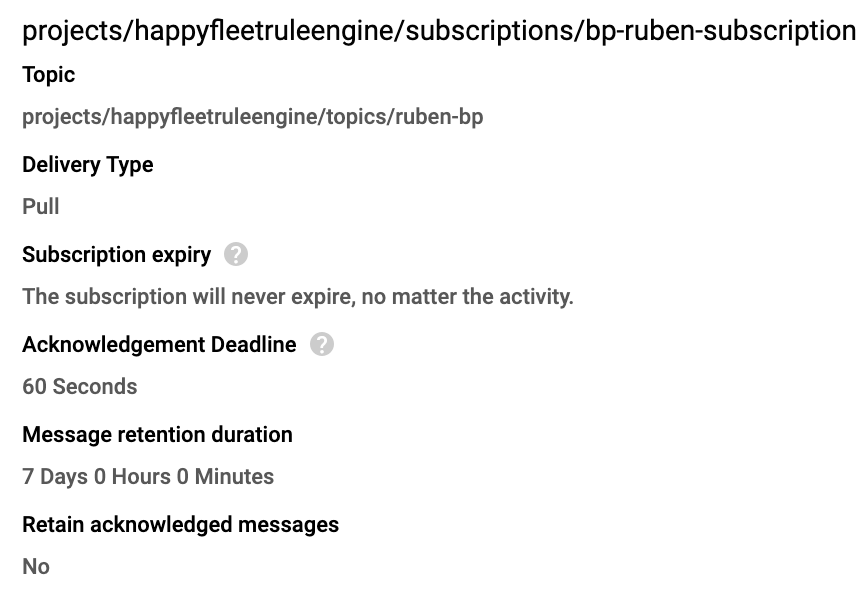
\includegraphics[width=140mm]{../gpsConfig.png}
    \caption{Configuratie van de topic voor de gebruikte subscription}
    
\end{figure}
\subsubsection{GooglePubSubConfig}
Voor Google Pub/Sub is de configuratie iets afwijkend in vergelijking met Kafka en RabbitMq. Hier gebruiken we zowel een configuration klasse als de application.yml file. De configuratie klasse wordt aangeduid met de annotatie van Spring: @Configuration. Ook de application.yml file wordt gebruikt voor drie properties. Laat ons eerst de application.yml file overlopen. Deze wordt gebruikt om de naam van de topic in op te slaan, zodat deze niet voorkomt in onze code. Dan zijn er nog twee zaken die hier geconfigureerd worden: spring.cloud.gcp.project.id en spring.cloud.gcp.credentials.location. Het eerste is het project id van het cloud platform waar uw Pub/Sub zich bevindt. Het tweede is het path naar de credentials file om toegang te krijgen tot het cloud platform. De rest van het configuratiewerk wordt in de GooglePubSubConfig klasse gedaan. De eerste methode createBachelorproefChannelOutput geeft een MessageChannel terug. Deze heeft een annotatie @Bean die de naam 'bachelorproef-channel-output'' krijgt. Dit is letterlijk het 'kanaal' dat we gaan gebruiken om onze messages te verzenden. De volgende methode geeft een MessageHandler terug en meer bepaald in dit geval een PubSubMessageHandler. Deze heeft een pubsubTemplate die je kan vergelijken met de kafkaTemplate of rabbitTemplate. Ook wordt er verwacht dat je de naam van uw topic meegeeft. Naar deze topic zal hij de messages sturen. Zoals te zien is gebruiken we weer de @Value annotatie van het Spring framework om de naam van onze topic niet in onze code te moeten plaatsen. Boven deze methode zie je niet alleen de annotatie @Bean maar ook @ServiceActivator met de naam van de bean uit de eerste methode. Dit zal ik zo meteen uitleggen wanneer we aan het stukje komen van de GooglePubSubPublisher interface. De derde methode returned een JacksonPubSubMessageConverter. Door deze bean aan te maken weet Spring automatisch dat hij deze klasse moet gebruiken om onze objecten om te zetten naar het Json-formaat.

 \begin{lstlisting}[language = Java , frame = trBL , firstnumber = 1 , escapeinside={(*@}{@*)}]
@Configuration
public class GooglePubSubConfig {
    
    @Bean("bachelorproef-channel-output")
    public MessageChannel createBachelorproefChannelOutput() {
        return new DirectChannel();
    }
    
    @Bean
    @ServiceActivator(inputChannel = "bachelorproef-channel-output")
    public MessageHandler messageSender(
    PubSubOperations pubsubTemplate,
    @Value("${pubsub.topic}") String topicName
    ) {
        return new PubSubMessageHandler(pubsubTemplate, topicName);
    }
    
    @Bean
    public JacksonPubSubMessageConverter createJacksonMessageConverter(final ObjectMapper objectMapper) {
        return new JacksonPubSubMessageConverter(objectMapper);
    }
    
}
     \end{lstlisting}
\subsubsection{GooglePubSubPublisher}
Deze klasse heeft maar één methode, namelijk publishData. Deze methode verstuurt het Data-object naar de topic via het kanaal \emph{bachelorproef-channel-output}. Er hoeft geen implementatie te zijn van deze methode, het Spring-framework regelt al het andere werk in jouw plaats. Maar toch is het handig om even te verduidelijken hoe dit allemaal in zijn werk gaat. Wanneer de methode publishData met een Data object opgeroepen wordt, dan verzendt hij deze data via het kanaal dat beschreven staat in de annotatie @MessagingGateway. Maar deze interface kan dit werk niet op zijn eentje doen en zoekt daarom hulp in de configuratie. Als we dan teruggaan naar de GooglePubSubConfig klasse, dan zien we boven de methode die een MessageHandler teruggeeft de @ServiceActivator staan en dezelfde naam van het kanaal. Dus om kort samen te vatten: als de methode publishData opgeroepen wordt, dan kijkt hij welk kanaal hij nodig heeft om te verzenden. Dan zoekt hij een MessageHandler die geactiveerd wordt wanneer zijn kanaal gebruikt wordt en deze handler gebruikt spring om de message dan effectief te verzenden. Omdat de bean die de MessageChannel teruggeeft de naam ''bachelorproef-channel-output'' heeft, en deze naam van het kanaal ook in de annotatie @ServiceActivator staat, weet Spring dat dit kanaal moet gebruikt worden.

 \begin{lstlisting}[language = Java , frame = trBL , firstnumber = 1 , escapeinside={(*@}{@*)}]
@MessagingGateway(defaultRequestChannel = "bachelorproef-channel-output")
@Component
public interface GooglePubSubPublisher {
    void publishData(Data data);
    
}
     \end{lstlisting}
     
\subsection{Creëren van de data}
Nu de drie technologieën klaar zijn om data te verzenden, blijft er voor deze applicatie alleen nog het creëren van de data en het verzenden ervan over. Er zijn nog drie cruciale elementen die besproken moeten worden en die zijn: de ProducerApplication- , de RandomDataProvider- en de RandomDataPublisher.

\subsubsection{ProducerApplication}
Dit is de eerste klasse die gebruikt wordt om de applicatie te starten. In de methode runner geven we via de parameters alle klassen mee die data publishen. Dit is dus een object van de klasse voor Google Pub/Sub, Kafka en RabbitMq. Ook moeten we de klasse RandomDataPublisher meegeven. In deze methode roep je de methode doStuff op van de RandomDataPublisher klasse. Wat deze methode exact doet bespreken we later. Maar je moet meegeven welke publisher je wilt gebruiken. Deze lijn code is het enige dat je moet aanpassen om data te verzenden voor één van de drie technologieën.

\begin{lstlisting}[language = Java , frame = trBL , firstnumber = 1 , escapeinside={(*@}{@*)}]
@SpringBootApplication
@Slf4j
public class ProducerApplication {
    
    public static void main(String[] args) {
        SpringApplication.run(ProducerApplication.class, args);
    }
    
    @Bean
    public CommandLineRunner runner(final RandomDataPublisher randomDataPublisher,
        final GooglePubSubPublisher googlePubSubPublisher,
        final KafkaPublisher kafkaPublisher,
        final RabbitMqPublisher rabbitMqPublisher) {
            return args -> {
              randomDataPublisher.doStuff(googlePubSubPublisher);
              //   OF:         randomDataPublisher.doStuff(kafkaPublisher);
              //   OF;         randomDataPublisher.doStuff(rabbitMqPublisher);
        };
    }
}
     \end{lstlisting}
\subsubsection{RandomDataProvider}
Deze klasse is een hulpklasse die de lijst van Data objecten genereert. Het aantal objecten wordt meegegeven als parameter en wordt ingesteld in de RandomDataPublisher. De naam van het object en de beschrijving is telkens de naam van het attribuut, respectievelijk name en description, plus het id eraan geplakt. Hier wordt ook een nieuwe datum gecreëerd die dient als sendedDate.
\begin{lstlisting}[language = Java , frame = trBL , firstnumber = 1 , escapeinside={(*@}{@*)}]
@Component
public class RandomDataProvider {
    public List<Data> create(int numberOfEntries) {
        final List<Data> dataList = new ArrayList<>();
        for (int i = 0; i < numberOfEntries; i++) {
            dataList.add(new Data(i, "name" + i, "description" + i, new Date()));
        }
        
        return dataList;
    }
}
           \end{lstlisting}

\subsubsection{RandomDataPublisher}
Deze klasse heeft de functionaliteit om de methode create uit de klasse RandomDataProvider op te roepen om de Data objecten te genereren en door te geven aan de juiste publisher. De constructor heeft opnieuw de publisher klassen als parameter die gecreëerd worden door Spring Boot. Het heeft ook nog een extra parameter namelijk een instantie van de RandomDataProvider om later de create methode te kunnen gebruiken.

We verdiepen ons even in de methode doStuff. Hierin wordt aan de randomDataProvider gevraagd om een aantal Data objecten te maken. In dit codevoorbeeld is dit 10000 objecten. Deze slaat hij op een lijst van het type Data. In de methode wordt er gecontroleerd van welke instantie de publisher is die je mee krijgt. Indien de publisher van Kafka of RabbitMq is dan wordt deze lijst verzonden naar de Kafka topic of de RabbitMq exchange. Is het een instantie van de publisher van Google Pub/Sub dan wordt deze lijst overlopen en per object verstuurd. De publish methode van GooglePubSubPublisher wenst maar één object en geen lijst van objecten.

\begin{lstlisting}[language = Java , frame = trBL , firstnumber = 1 , escapeinside={(*@}{@*)}]
@Component
public class RandomDataPublisher {
    
    private final RandomDataProvider randomDataProvider;
    private final KafkaPublisher kafkaPublisher;
    private final GooglePubSubPublisher googlePubSubPublisher;
    private final RabbitMqPublisher rabbitMqPublisher;
    
    public RandomDataPublisher(RandomDataProvider randomDataProvider,
    KafkaPublisher kafkaPublisher,
    GooglePubSubPublisher googlePubSubPublisher,
    RabbitMqPublisher rabbitMqPublisher) {
        this.randomDataProvider = randomDataProvider;
        this.kafkaPublisher = kafkaPublisher;
        this.googlePubSubPublisher = googlePubSubPublisher;
        this.rabbitMqPublisher = rabbitMqPublisher;
    }
    
    public void doStuff(Object object) {
        final List<Data> dataList = randomDataProvider.create(10_000);
        if(object instanceof GooglePubSubPublisher) {
            for (Data data : dataList) {
                googlePubSubPublisher.publishData(data);
                System.out.printf("publishing data: %s", data);
            }
        } else if (object instanceof KafkaPublisher){
            kafkaPublisher.publish(dataList);
        } else {
            rabbitMqPublisher.publish(dataList);
        }
        
    }
}
\end{lstlisting}

\section{Consumer project}
De bedoeling van deze applicatie is dat ze wanneer er iets op een topic of queue geplaatst wordt, ze deze informatie weer omzet en opslaat in een lokale databank. Bij het opslaan van de data wordt er meer opgeslagen dan dat er informatie binnenkomt om deze te kunnen vergelijken, maar dit wordt straks duidelijker. Wanneer deze applicatie opgestart is, luistert deze voortdurend naar de topics, of naar de queue, of er messages op geplaatst worden. Indien er een message op een topic of de queue toegekomen is, dan leest hij deze meteen uit. Deze applicatie luistert dus tegelijkertijd naar zowel de topic van Kafka en Google Pub/Sub als naar de queue van RabbitMq. Om dit niet met elkaar te laten beïnvloeden wordt tijdens dit onderzoek enkel data verstuurd van een bepaalde technologie, bijvoorbeeld Kafka, indien de consumerapplicatie niets meer leest van een andere technologie. Deze aanpak zorgt er dus voor dat data van verschillende technologieën niet door elkaar gelezen worden. We hebben in deze applicatie hetzelfde domein object van de klasse Data, want we willen het object dat verstuurd werd op dezelfde manier terugkrijgen. Door later de juiste deserializers mee te geven, moeten we ons geen zorgen maken en wordt het inkomende object automatisch gemapt naar hetzelfde domeinobject.
\begin{lstlisting}[language = Java , frame = trBL , firstnumber = 1 , escapeinside={(*@}{@*)}]
@Getter
@AllArgsConstructor
@NoArgsConstructor
@ToString
public class Data {
    private int id;
    private String name;
    private String description;
    private Date sendedDate;
}
\end{lstlisting}

Naast deze Data klasse hebben we ook per technologie een entity klasse en repository. De entity klasse zorgt ervoor dat per technologie een tabel gecreëerd wordt in de databank. De repository zorgt ervoor dat een object van deze klasse effectief opgeslagen kan worden. De namen van deze entity klassen zijn: DataGPS, DataKafka en DataRMQ. Voor de repository zijn de namen van de interfaces: DataGPSRepository, DataKafkaRepository en DataRMQRepository. De implementatie van deze klassen is telkens dezelfde, maar het is nodig om deze apart te houden verschillende tabellen te hebben in de databank per technologie. Hier zullen we één entity klasse en repository uitleggen want voor de andere is het analoog.

\subsubsection{Entity klasse}
We bekijken het voorbeeld van de DataGPS klasse.
\begin{lstlisting}[language = Java , frame = trBL , firstnumber = 1 , escapeinside={(*@}{@*)}]
@Entity
public class DataGPS {
    
    public DataGPS( int dataId, String name, String description, Date sendedDate, Date receivedDate, long timeDiff) {
        this.dataId = dataId;
        this.name = name;
        this.description = description;
        this.sendedDate = sendedDate;
        this.receivedDate = receivedDate;
        this.timeDiff = timeDiff;
    }
    
    @Id
    @GeneratedValue(strategy = GenerationType.IDENTITY)
    private long id;
    
    private int dataId;
    private String name;
    private String description;
    private Date sendedDate;
    private Date receivedDate;
    private long timeDiff;
}
\end{lstlisting}
Boven de klasse staat er een annotatie uit de package javax.persistence. De @Entity zorgt ervoor dat van deze klasse automatisch een tabel aangemaakt wordt in de databank. De attributen van deze klasse zullen automatisch ook de velden zijn van deze tabel.

In de constructor zien we dat alle attributen van deze klasse aanwezig zijn als parameter, behalve het attribuut id. Dit is niet nodig om in de constructor mee te geven aangezien deze waarde automatisch gecreëerd wordt. Door de annotatie @Id zeg je dat dit veld het id is van de tabel en dus uniek moet zien. Dit is eveneens de primary key van de tabel. Door de tweede annotatie @GeneratedValue zorg je ervoor dat er automatisch een waarde aangemaakt wordt die uniek is. Je moet je dus voor de rest niets meer aantrekken van dit attribuut.

\subsubsection{Repository}
Ook hier bekijken we het voorbeeld van de DataGPSRepository.
\begin{lstlisting}[language = Java , frame = trBL , firstnumber = 1 , escapeinside={(*@}{@*)}]
public interface DataGPSRepository extends CrudRepository<DataGPS, Long> {
}
\end{lstlisting}
Op het eerste zicht lijkt het alsof deze klasse geen implementatie heeft. Toch kan je bij deze repository bijvoorbeeld de methode save(DataGPS data) oproepen om een object van de klasse DataGPS op te slaan. Dit komt omdat deze interface extends van de interface CrudRepository<T, ID>. Deze interface zorgt ervoor dat je op een object van de klasse, die je meegeeft in de plaats van T, de basisoperaties kan uitvoeren zoals save.

\subsection{Kafka}
\subsubsection{KafkaConfig}
Eerst en vooral zijn er opnieuw enkele waardes die we liever niet weergeven. In dit geval zijn er vier waardes: de  naam van de topic, het bootstrapadres (het adres waar de server zich bevindt), een key en een secret. Sommige van deze variabelen zullen gebruikt worden in de application.yml file waar ook deze vier waardes zich bevinden. Anderen, zoals de topic, worden dan weer gebruikt in de implementatie zelf. De namen die we aan deze variabelen gegeven hebben in dit project zijn: kafka.topic.name (voor de naam van de topic), kafka.bootstrapAddress (voor het bootstrapadres), kafka\textunderscore key en kafka\textunderscore secret (voor de key en de secret).

Verder wordt er voor de configuratie enkel de application.yml gebruikt en dus geen aparte KafkaConfig klasse. Dit is hoe de configuratie er uit ziet voor Kafka:
\begin{lstlisting}[language = xml , frame = trBL , firstnumber = 1 , escapeinside={(*@}{@*)}]
spring:
    kafka:
        consumer:
            bootstrap-servers: ${kafka.bootstrapAddress}
            group-id: foo
            auto-offset-reset: latest
            key-deserializer: org.apache.kafka.common.serialization.StringDeserializer
            value-deserializer: org.apache.kafka.common.serialization.StringDeserializer

        properties:
            ssl.endpoint.identification.algorithm: https
            sasl.mechanism: PLAIN
            request.timeout.ms: 20000
            retry.backoff.ms: 500
            sasl.jaas.config: org.apache.kafka.common.security.plain.PlainLoginModule required username="${kafka_key}" password="${kafka_secret}";
            security.protocol: SASL_SSL
\end{lstlisting}

We zien dat het bootstrapadres meegegeven wordt. Op deze manier weet de applicatie op welke server hij moet gaan zoeken. Hier worden er geen serializers gebruikt maar deserializers, wat voor zich spreekt. Om de waarde van de Json te deserializeren wordt de StringDeserializer gebruikt uit de package org.apache.kafka.common.serialization. Om de key te deserializeren wordt de StringDeserializer gebruikt uit dezelfde package. Verder hoeven we ons geen zorgen te maken over het deserializeren. Het Spring framework regelt al dit werk voor ons. We kunnen er dus van uit gaan dat als er een message binnen komt dit automatisch op een goede manier omgezet wordt. Verder zien we ook dat de kafka\textunderscore key en kafka\textunderscore secret variabelen gebruikt worden om het wachtwoord en gebruikersnaam mee te geven.

\subsubsection{KafkaReceiver}
Deze klasse is verantwoordelijk voor het ontvangen van objecten die van de Kafka topic komen. Deze klasse heeft twee attributen, een ObjectMapper en de DataKafkaRespository om de objecten op te slaan in de databank. Door deze mee te geven als parameter in de constructor zorgt Spring Boot er opnieuw voor dat deze automatisch gecreëerd worden.

Deze klasse bevat slechts één methode: listen(String message). Hier zien we dat er boven de annotatie @KafkaListener te lezen valt. Deze annotatie krijgt de naam van de topic mee en het groupId. Hierdoor weet de applicatie van waar hij berichten moet lezen. Door deze annotatie zeg je dat als er een bericht uitgelezen moet worden uit deze topic, dat je deze methode moet uitvoeren. De String die de methode meekrijgt als parameter werd al automatisch gedeserialiseerd door de configuratie in application.yml. 

In deze methode lezen we via de objectMapper de message uit en vormen deze om naar ons domeinobject van het type Data, dat dezelfde klasse is als bij de producer applicatie. Hierna maken we een nieuwe datum aan om te registreren wat de tijd was van het uitlezen van de message. Hierna vragen we aan ons object wat de tijd was van verzenden. Dit trekken we van elkaar af en op deze manier komen we te weten hoeveel milliseconden het verschilt tussen het uitlezen van de message en het verzenden ervan. Vervolgens slaan we deze gegevens op als een object van de klasse DataKafka. Veel van deze informatie halen we uit de oorspronkelijke message van het type Data. Maar voor de analyse van dit onderzoek is het ook handig om extra attributen mee te geven zoals het verschil. Daarna wordt de methode save uit de repository uitgevoerd. Op deze manier wordt dit object opgeslagen in de databank.

\begin{lstlisting}[language = java , frame = trBL , firstnumber = 1 , escapeinside={(*@}{@*)}]
@Component
public class KafkaReceiver {
    
    private ObjectMapper objectMapper;
    private DataKafkaRepository dataKafkaRepository;
    
    public KafkaReceiver(final ObjectMapper objectMapper,
    final DataKafkaRepository dataKafkaRepository) {
        this.objectMapper = objectMapper;
        this.dataKafkaRepository = dataKafkaRepository;
    }
    
    @KafkaListener(topics = "${kafka.topic.name}", groupId = "foo")
    public void listen(String message) throws Exception {
        
        try {
            Data data = objectMapper.readValue(message, Data.class);
            System.out.println(data);
            
            Date received = new Date();
            Date sended = data.getSendedDate();
            
            long difference = received.getTime() - sended.getTime();
            
            dataKafkaRepository.save(new DataKafka(data.getId(), data.getName(), data.getDescription(), data.getSendedDate(),received, difference));
        } catch (IOException e) {
            e.printStackTrace();
        }
        
        System.out.println("Received Messasge in group foo: " + message);
    }
}
\end{lstlisting}
\subsection{RabbitMq}
\subsubsection{RabbitMqConfig}
Ook hier wordt er enkel gebruikt gemaakt van de application.yml om RabbitMq te configureren. Eerst en vooral zijn er ook hier enkele variabelen die we liever niet blootstellen, zoals de naam van de queue. Deze zal gebruikt worden tijdens de implementatie in de klasse RabbitMqReceiver. Hiernaast willen we ook de username,  password en het hostadres niet tonen. Deze zullen gebruikt worden in deze application.yml file. De namen van deze variabelen zijn respectievelijk: rabbitmq\textunderscore queue\textunderscore name, rabbitmq\textunderscore username, rabbitmq\textunderscore password en rabbitmq\textunderscore host. 

De rest van de configuratie ziet er als volgt uit: 
\begin{lstlisting}[language = xml , frame = trBL , firstnumber = 1 , escapeinside={(*@}{@*)}]
spring:
    rabbitmq:
        host: ${rabbitmq_host}
        port: 16379
        username: ${rabbitmq_username}
        password: ${rabbitmq_password}
        virtual-host: "rabbitmq"
        ssl:
            enabled: true
            algorithm: "TLSv1.2"
        listener:
            simple:
                default-requeue-rejected: false
            direct:
                default-requeue-rejected: false
\end{lstlisting}

Je ziet dat het hostadres meegegeven wordt, alsook de username en password.
\subsubsection{RabbitMqReceiver}
Deze klasse is zo goed als gelijk aan de KafkaReceiver. Het is evident dat de DataKafkaRepository vervangen is door de DataRMQRespository. Boven de methode receiveMessage staat ook een andere notatie namelijk @RabbitListener. Door deze annotatie boven de methode te zetten, weet de applicatie dat hij deze methode moet uitvoeren als er op de opgegeven queue een bericht komt. In deze methode wordt de message eerst weer omgezet in een Data object en dan opgeslagen als een DataRMQ object met de waardes van de message en het verschil tussen het verzenden en het ontvangen.
\begin{lstlisting}[language = java , frame = trBL , firstnumber = 1 , escapeinside={(*@}{@*)}]
@Component
public class RabbitMqReceiver {
    
    private ObjectMapper objectMapper;
    
    private DataRMQRepository dataRMQRepository;
    
    public RabbitMqReceiver(final ObjectMapper objectMapper,
    final DataRMQRepository dataRMQRepository) {
        this.objectMapper = objectMapper;
        this.dataRMQRepository = dataRMQRepository;
    }
    
    @RabbitListener(queues = "${rabbitmq_queue_name}")
    public void receiveMessage(String message) throws Exception {
        try {
            Data data = objectMapper.readValue(message, Data.class);
            System.out.println(data);
            
            Date received = new Date();
            Date sended = data.getSendedDate();
            
            long difference = received.getTime() - sended.getTime();
            
            dataRMQRepository.save(new DataRMQ(data.getId(), data.getName(), data.getDescription(), data.getSendedDate(),received, difference));
        } catch (IOException e) {
            e.printStackTrace();
        }
        System.out.println("Receiving message RabbitMq: " + message);
    }
   
}
\end{lstlisting}
\subsection{Google Pub/Sub}
\subsubsection{GooglePubSubConfig}
Voor Google Pub/Sub werken we met een config klasse en ook met de application.yml. Er zijn vier zaken die meegegeven worden in deze laatste file. Twee ervan worden gebruikt in de implementatie, de andere twee moet je gewoon meegeven in deze file. De twee die gebruikt worden in de implementatie zijn pubsub.subscription en pubsub.autostartup. De eerste is de naam van de subscription, de tweede is een boolean om aan te duiden of de subscriber moet starten met luisteren als de applicatie wordt opgestart of niet. De andere twee configuraties die je moet meegeven zijn: spring.cloud.gcp.project-id en spring.cloud.gcp.credentials.location. De eerste is het id van het project, de tweede is de plaats waar de credentials staan om te kunnen inloggen op het Google Cloud Platform. 

De GooglePubSubConfig klasse ziet er als volgt uit:
\begin{lstlisting}[language = java , frame = trBL , firstnumber = 1 , escapeinside={(*@}{@*)}]
@Configuration
public class GooglePubSubConfig {
    
    @Bean("bachelorproef-channel-input")
    public MessageChannel createDeviceEventChannelInput() {
        return new DirectChannel();
    }
    
    @Bean
    public PubSubInboundChannelAdapter createDeviceChannelAdapter(
    PubSubOperations pubSubTemplate,
    @Value("${pubsub.subscription}") String subsciptionName,
    @Qualifier("bachelorproef-channel-input") MessageChannel inputChannel,
    @Value("${pubsub.autostartup}") Boolean autoStart) {
        
        final PubSubInboundChannelAdapter adapter = new PubSubInboundChannelAdapter(pubSubTemplate, subsciptionName);
        adapter.setOutputChannel(inputChannel);
        adapter.setAckMode(AckMode.AUTO);
        adapter.setPayloadType(Data.class);
        adapter.setAutoStartup(autoStart);
        return adapter;
    }
    
    @Bean
    public JacksonPubSubMessageConverter createJacksonMessageConverter(final ObjectMapper objectMapper) {
        return new JacksonPubSubMessageConverter(objectMapper);
    }
\end{lstlisting}
Boven de klasse ziet u opnieuw de annotatie @Configuration staan om aan te geven aan het Spring framework dat dit een configuratie is. Verder wordt er een nieuwe MessageChannel aangemaakt. Dit is het 'kanaal' die gebruikt wordt om messages te ontvangen. Er wordt ook een naam gegeven aan dit kanaal namelijk ''bachelorproef-channel-input''. Vervolgens moet er een PubSubInboundChannelAdapter aangemaakt worden die enkele configuraties bevat. Als parameter van deze methode moet je een PubSubOperations meegeven, dit is te vergelijken met de KafkaTemplate of RabbitTemplate. Verder moet je de naam van de subscription meegeven en ook welke MessageChannel hij moet gebruiken om messages te ontvangen. Via de @Qualifier annotatie zeg je dat hij de MessageChannel moet gebruiken die we daarnet aangemaakt hebben. Als laatste geef je dan nog mee of het starten met luisteren naar de topic automatisch moet gebeuren of niet. In deze methode stel je dan nog in dat de payload van de message, die een Json is, van het type Data is. Door de laatste methode, die een JacksonPubSubMessageConverter aanmaakt, kan deze Json automatisch omgezet worden in een instantie van Data.
\subsubsection{GooglePubSubReceiver}
Dit doet ongeveer hetzelfde als de vorige receivers. Alleen hoef je hier geen ObjectMapper te gebruiken omdat deze al is meegegeven aan de JacksonPubSubMessageConverter. Verder wordt er gebruik gemaakt van de DataGPSRepository om objecten van het type DataGPS op te slaan. 

De methode storeData krijgt geen message mee in de vorm van een String, want het omzetten van de message naar een object van Data is al gebeurd door de JacksonPubSubMessageConverter. Je hebt dus meteen het Data object dat binnenkomt. Je hoeft dus enkel maar de juiste waardes op te vragen en mee te geven aan een nieuw object van de klasse DataGPS. Ook hier werd het verschil berekend tussen het verzenden en het ontvangen. Boven de methode staat de annotatie @ServiceActivator die als parameter het kanaal heeft waar messages op toekomen. Dit wil zeggen als een message langs dit kanaal binnenkomt, dat de applicatie deze methode moet uitvoeren.
\begin{lstlisting}[language = java , frame = trBL , firstnumber = 1 , escapeinside={(*@}{@*)}]
@Component
public class GooglePubSubReceiver {
    
    private DataGPSRepository dataGPSRepository;
    
    public GooglePubSubReceiver(final DataGPSRepository dataGPSRepository) {
        this.dataGPSRepository = dataGPSRepository;
    }
    
    @ServiceActivator(inputChannel = "bachelorproef-channel-input")
    public void storeData(final Data data) throws Exception {
        System.out.println("--- Getting data: name: " + data.getName() + ", description: " + data.getDescription() +
        ", id: " + data.getId() + ", sended: " + data.getSendedDate().toString() + ", received: " + new Date().toString() + " ---");
        
        
        Date received = new Date();
        Date sended = data.getSendedDate();
        
        long difference = received.getTime() - sended.getTime();
        
        dataGPSRepository.save(new DataGPS(data.getId(), data.getName(), data.getDescription(), data.getSendedDate(), received, difference));
    }
    
}
\end{lstlisting}
\section{Onderzoek}
Zoals al eerder vermeld worden de resultaten opgeslagen in een databank. De databank draait lokaal in een Docker container. Dit is de eenvoudige configuratie die nodig is om te databank op te stellen:
\begin{lstlisting}[language = xml , frame = trBL , firstnumber = 1 , escapeinside={(*@}{@*)}]
spring:
    datasource:
        url: "jdbc:postgresql://localhost:5432/postgres"
        username: postgres
        password: postgres
    jpa:
        hibernate:
            ddl-auto: create
        jdbc:
            lob:
                non-contextual-creation: true
\end{lstlisting}
De URL van de databank wordt meegegeven met daarachter de naam van de databank. Daaronder geef je de gebruikersnaam en wachtwoord mee. Het is niet erg dat het wachtwoord bloot gegeven wordt, want dit is toch een lokale databank. Verder zie je ook dat indien de applicatie opnieuw opstart, de database opnieuw gecreëerd wordt.

Verder werd dit onderzoek drie keer uitgevoerd. Een keer met 10000, 100000 en 1000000 Data objecten die verzonden werden. Zo kunnen we ook vergelijken hoe sterk het tijdsverschil wordt. De bedoeling was om de methodes die de objecten ontvangen zo klein mogelijk te houden. Want hoe groter deze methodes worden, hoe langer het duurt per object om deze objecten te ontvangen en dit zou een verkeerd beeld kunnen geven.

De resultaten werden per technologie opgeslagen in een CSV-file om daarna berekeningen op te kunnen doen. Dit werd gedaan met een Python script. 

Eerst wordt de CSV uitgelezen via de pandas library. Hierna wordt er wat aan data exploratie gedaan om te controleren of de waardes die uitgelezen werden wel effectief mogelijk zijn. 
\begin{lstlisting}[language = python , frame = trBL , firstnumber = 1 , escapeinside={(*@}{@*)}]
import pandas as pd
result = pd.read_csv('/Users/rubendesmet/Desktop/gps10_000.csv',sep=',')
print(result.head())
print(result.columns)
print(result.index)
print(result.count())
print(result.shape)
\end{lstlisting}

Vervolgens worden de kolommen die niet van toepassing zijn verwijderd. Enkel de kolom timeDiff zou moeten overblijven die het verschil van de ontvangen en verzonden tijd voorstelt. Daarna kijken we hoeveel rijen er in de tabel zitten, worden eventuele NaN verwijderd, en kijken we nog eens hoeveel rijen er in de tabel zitten. Als laatste controlemiddel printen we nog eens de eerste vijf rijen af en zo kunnen we ook zien of we kolommen vergeten verwijderen zijn. 

\begin{lstlisting}[language = python , frame = trBL , firstnumber = last , escapeinside={(*@}{@*)}]
print(result.count())
result = result.dropna()
print(result.count())
print(result.head())
\end{lstlisting}

Dan rest ons nog één ding, namelijk het berekenen van het gemiddelde van deze kolom, samen met het minimum en maximum.
\begin{lstlisting}[language = python , frame = trBL , firstnumber = last , escapeinside={(*@}{@*)}]
print(result['timeDiff'].mean())
print(result['timeDiff'].max())
print(result['timeDiff'].min())
\end{lstlisting}
Al deze stappen worden dus negen keer uitgevoerd. Drie keer per technologie en drie keer per hoeveelheid verzonden data.

\subsubsection{Tweede deel van het onderzoek}
Nadat dit allemaal onderzocht was, werd er door beslist door het bedrijf TVH dat we ook nog de gebruikte memory zouden onderzoeken. Hiervoor moest er niets aangepast worden aan de producer applicatie, maar wel aan de consumer applicatie. 

\begin{lstlisting}[language = python , frame = trBL , firstnumber = last , escapeinside={(*@}{@*)}]
// Get the Java runtime
Runtime runtime = Runtime.getRuntime();
// Run the garbage collector
runtime.gc();
// Calculate the used memory
long memory = runtime.totalMemory() - runtime.freeMemory();

memory = bytesToMegabytes(memory);
\end{lstlisting}
Per receiver werd deze code toegevoegd in de methode die de messages ontvangt. Deze code achterhaalt de gebruikte memory. De hulpmethode bytesToMegabytes(memory) zet de memory om naar megabytes. Dit resultaat werd dan ook meegegeven bij het aanmaken van een object van een entity en zo mee opgeslagen. Dit wil zeggen dat er in DataGPS, DataKafka en DataRMQ een attribuut memory bijkwam. Bij de resultaten van dit gedeelte van het onderzoek werd enkel rekening gehouden met de memory. Kijken naar het verschil tussen het verzenden en ontvangen in tijd was niet meer nodig. Het ophalen van het gebruik van memory neemt namelijk zo veel tijd in beslag dat het tijdsverschil niet meer relevant was om te bekijken.

Door dit nieuwe gedeelte van het onderzoek kwamen er 3 CSV bestanden bij. Eén bestand per technologie die de memory berekent. Er werd gekozen om telkens maar 1000 objecten te verzenden. Er kwamen dus ook drie nieuwe Python-scripts bij. Ook één per technologie die het gemiddelde, maximum en minimum van de memory berekende per technologie. Het opbouwen van deze scripts is gelijkaardig met het berekenen van het gemiddelde tijdsverschil. Maar in plaats van het tijdsverschil werd enkel de kolom met de memory bijgehouden.  